\documentclass{article}
\usepackage{minted}
\usepackage{listings}
\usepackage{graphicx}
\usepackage{physics}
\usepackage{siunitx}
\usepackage{placeins}

\usepackage{lmodern}
\usepackage{amssymb,amsmath}
\usepackage{ifxetex,ifluatex}
\usepackage{fixltx2e} % provides \textsubscript
\ifnum 0\ifxetex 1\fi\ifluatex 1\fi=0 % if pdftex
  \usepackage[T1]{fontenc}
  \usepackage[utf8]{inputenc}
  \usepackage{textcomp} % provides euro and other symbols
\else % if luatex or xelatex
  \usepackage{unicode-math}
  \defaultfontfeatures{Ligatures=TeX,Scale=MatchLowercase}
\fi
% use upquote if available, for straight quotes in verbatim environments
\IfFileExists{upquote.sty}{\usepackage{upquote}}{}
% use microtype if available
\IfFileExists{microtype.sty}{%
\usepackage[]{microtype}
\UseMicrotypeSet[protrusion]{basicmath} % disable protrusion for tt fonts
}{}
\IfFileExists{parskip.sty}{%
\usepackage{parskip}
}{% else
\setlength{\parindent}{0pt}
\setlength{\parskip}{6pt plus 2pt minus 1pt}
}
\usepackage{hyperref}
\hypersetup{
            pdfborder={0 0 0},
            breaklinks=true}
\urlstyle{same}  % don't use monospace font for urls
\usepackage{color}
\usepackage{fancyvrb}
\newcommand{\VerbBar}{|}
\newcommand{\VERB}{\Verb[commandchars=\\\{\}]}
\DefineVerbatimEnvironment{Highlighting}{Verbatim}{commandchars=\\\{\}}
% Add ',fontsize=\small' for more characters per line
\newenvironment{Shaded}{}{}
\newcommand{\AlertTok}[1]{\textcolor[rgb]{1.00,0.00,0.00}{\textbf{#1}}}
\newcommand{\AnnotationTok}[1]{\textcolor[rgb]{0.38,0.63,0.69}{\textbf{\textit{#1}}}}
\newcommand{\AttributeTok}[1]{\textcolor[rgb]{0.49,0.56,0.16}{#1}}
\newcommand{\BaseNTok}[1]{\textcolor[rgb]{0.25,0.63,0.44}{#1}}
\newcommand{\BuiltInTok}[1]{#1}
\newcommand{\CharTok}[1]{\textcolor[rgb]{0.25,0.44,0.63}{#1}}
\newcommand{\CommentTok}[1]{\textcolor[rgb]{0.38,0.63,0.69}{\textit{#1}}}
\newcommand{\CommentVarTok}[1]{\textcolor[rgb]{0.38,0.63,0.69}{\textbf{\textit{#1}}}}
\newcommand{\ConstantTok}[1]{\textcolor[rgb]{0.53,0.00,0.00}{#1}}
\newcommand{\ControlFlowTok}[1]{\textcolor[rgb]{0.00,0.44,0.13}{\textbf{#1}}}
\newcommand{\DataTypeTok}[1]{\textcolor[rgb]{0.56,0.13,0.00}{#1}}
\newcommand{\DecValTok}[1]{\textcolor[rgb]{0.25,0.63,0.44}{#1}}
\newcommand{\DocumentationTok}[1]{\textcolor[rgb]{0.73,0.13,0.13}{\textit{#1}}}
\newcommand{\ErrorTok}[1]{\textcolor[rgb]{1.00,0.00,0.00}{\textbf{#1}}}
\newcommand{\ExtensionTok}[1]{#1}
\newcommand{\FloatTok}[1]{\textcolor[rgb]{0.25,0.63,0.44}{#1}}
\newcommand{\FunctionTok}[1]{\textcolor[rgb]{0.02,0.16,0.49}{#1}}
\newcommand{\ImportTok}[1]{#1}
\newcommand{\InformationTok}[1]{\textcolor[rgb]{0.38,0.63,0.69}{\textbf{\textit{#1}}}}
\newcommand{\KeywordTok}[1]{\textcolor[rgb]{0.00,0.44,0.13}{\textbf{#1}}}
\newcommand{\NormalTok}[1]{#1}
\newcommand{\OperatorTok}[1]{\textcolor[rgb]{0.40,0.40,0.40}{#1}}
\newcommand{\OtherTok}[1]{\textcolor[rgb]{0.00,0.44,0.13}{#1}}
\newcommand{\PreprocessorTok}[1]{\textcolor[rgb]{0.74,0.48,0.00}{#1}}
\newcommand{\RegionMarkerTok}[1]{#1}
\newcommand{\SpecialCharTok}[1]{\textcolor[rgb]{0.25,0.44,0.63}{#1}}
\newcommand{\SpecialStringTok}[1]{\textcolor[rgb]{0.73,0.40,0.53}{#1}}
\newcommand{\StringTok}[1]{\textcolor[rgb]{0.25,0.44,0.63}{#1}}
\newcommand{\VariableTok}[1]{\textcolor[rgb]{0.10,0.09,0.49}{#1}}
\newcommand{\VerbatimStringTok}[1]{\textcolor[rgb]{0.25,0.44,0.63}{#1}}
\newcommand{\WarningTok}[1]{\textcolor[rgb]{0.38,0.63,0.69}{\textbf{\textit{#1}}}}
\setlength{\emergencystretch}{3em}  % prevent overfull lines
\providecommand{\tightlist}{%
  \setlength{\itemsep}{0pt}\setlength{\parskip}{0pt}}
\setcounter{secnumdepth}{0}
% Redefines (sub)paragraphs to behave more like sections
\ifx\paragraph\undefined\else
\let\oldparagraph\paragraph
\renewcommand{\paragraph}[1]{\oldparagraph{#1}\mbox{}}
\fi
\ifx\subparagraph\undefined\else
\let\oldsubparagraph\subparagraph
\renewcommand{\subparagraph}[1]{\oldsubparagraph{#1}\mbox{}}
\fi

% set default figure placement to htbp
\makeatletter
\def\fps@figure{htbp}
\makeatother

\graphicspath{{../figures/}}

\title{AMATH 582 Homework 2: Classic Rock and Roll Shredding}
\author{Brady Griffith}

\begin{document}
    \begin{center}
        \Large AMATH 582 Homework 2: Classic Rock and Roll Shredding \par
        \large Brady Griffith
    \end{center}

    \begin{abstract}
        Spectrograms made suing the Gabor transform provide insight into how a signal's spectrum changes with time. Musical scores are just instructions of which frequencies to play for a certain amount of time, so should be identifiable from the spectrogram. In this work, I do just that with clips from \textit{Sweet Child O' Mine} by Guns N' Roses and \textit{Comfortably Numb} by Pink Floyd. It was possible to identify the correct score for the guitar solo in the Guns N' Roses song. In the Pink Floyd song the bass riff could be fully identified, along with parts of the guitar solo.
    \end{abstract}

    \section{Introduction and Overview}
    In 1977, Ian Dury introduced the immortal phrase "Sex and drugs and rock and roll" declaring them to be "very good indeed". Only the third one is suitable for time series analysis, so rock and roll will be the subject of this work. The objective is to determine the score from clips from of songs \textit{Sweet Child O' Mine} by Guns N' Roses and \textit{Comfortably Numb} by Pink Floyd.

    The ability to make spectrograms is already built onto most audio editing software, so this project really is just a demonstration of the technique. This method does have the advantage of being able to choose the colormap used.

    \section{Theoretical Background}
    The fundamental tool for this analysis is the discrete Gabor transform. This gives a changing spectrum as over time by taking the fourier transform of a window around that a series of time steps. In the continuous form, the Gabor transform of a signal $f(t)$ is
    \begin{equation}
        \tilde{f}(t, \omega) = \int_{-\infty}^{\infty} f(\tau)\bar{g}(\tau  - t) e^{- i \omega \tau} \dd{\tau}
    \end{equation}
    where $g(\tau - t)$ is the windowing function.

    The choise of windowing function can have effects on the legibility of the spectrogram. One of the biggest considerations of a window function is the tradeoff between resolution in time, $\sigma_t$, and frequency, $\sigma_f$. The uncertainty principle conditions that 
    \begin{equation}
        \sigma_t^2 \sigma_f^2 \geq \frac{1}{16 \pi^2}.
    \end{equation}
    The minimum uncertainty is achieved by gaussian windows, which is why those will be used throughout the project.

    I also make use of frequency filtering to isolate the bass. Because sharp filters introduce ringing and other artifacts some care is taken with filter design. The bass is lower pitch than the other instruments, so a low pass filter is used. I make it fourth order ($-80 \textrm{dB}/\textrm{decade}$). The filter function is
    \begin{equation}
        H(f) = \left( \frac{1}{f/f_0 + 1} \right)^4
    \end{equation}
    where $f_0$ is the cutoff frequency.

    \section{Algorithm Implementation and Development}
    The first step is to import the songs in a way that gives a numpy array. I use the scikit-sound package, which gives an object with both the sound data as a numpy array, and the sample rate.

    The Gabor transform is preformed using the \lstinline{stft} function in the scipy signal package. I'd like to control slightly different parameters than the arguments of this function, so some processing is needed. The \lstinline{windows} parameter takes care of the gaussian window with the appropriate width. There is also \lstinline{nperseg} which is the size of the segment around each sample time to preform the transform over. It must be large enough that the gaussian has nearly gone to 0 by the edges. I use the nearest (in log space) power to two samples to 5 times the gaussian width. The time sampling frequency is handled by \lstinline{noverlap}, which is how much each window overlaps with the previous. I set this to be the segment width minus one quarter the gaussian width. This produces spectra every quarter gaussian width.

    There are 3 different spectrograms produced which each have a unique choice of window width. To examine the guitar riff in \textit{Sweet Child O' Mine}, the riff is at around 4 notes per seconds and requires a time resolution $ > 0.125 \si{s}$. The lowest note is $C4 \sharp$ at $277 \si{Hz}$ which requires a frequency resolution of $> 8 \si{Hz}$ to distinguish from the next note. This is more than easily satisfied by the uncertainty principle, so I split the difference in time/frequency and use $0.05 \si{s}$ window widths, which gives a $6.4 \si{Hz}$ frequency resolution.

    This tradeoff is somewhat more complicated for \textit{Comfortably Numb}. First I consider the bass riff which is within the range of $50 \si{Hz}$ to $110 \si{Hz}$ Hz. In order to distinguish notes at the low end, a resolution $>1.4 \si{Hz}$. However, the bass riff is mush slower than the others at around 60 BPM. For these reasons, a longer $0.1 \si{s}$ window is used.

    The guitar riff in that song has a some rapid variations, so a higher time resolution is needed. This requirement comes at the expense of higher frequency resolution, but as mentioned in the the first riff, it's still possible to reduce that and distinguish notes. A $.04 \si{s}$ window is used.

    The bass rift exists below $140 \si{Hz}$, so that is used for the low pass cutoff. The entire song is fourier transformed with the \lstinline{rfft} function in numpy. The filter is multiplied against this and the song is moved back into the time domain with \lstinline{irfft}. The array is converted into a sound object and exported as a wav file.
    
    \section{Computational Results}
    A spectrogram focusing on each of the three instruments is now presented. I make use of a SciVisColor wave colormap in order to highlight structure across the full range of intensities.

    \begin{figure}[tbp]
        \centering
        \includegraphics[width=.98\textwidth]{GNR-Spectrum.png}
        \caption{The spectrogram of the intro to \textit{Sweet Child O' Mine} by Guns N' Roses. This range highlights the guitar riff.}
        \label{fig:GNR}
    \end{figure}

    The first spectrogram is for \textit{Sweet Child O' Mine} and is in figure \ref{fig:GNR}. It is very easy to identify the notes of the riff. As I transcribed it, the score is:

    \begin{center}
        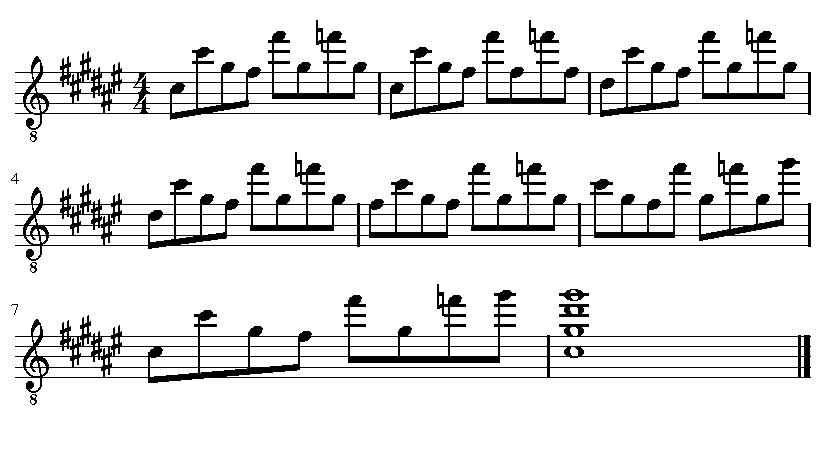
\includegraphics[width=.9\textwidth]{GNR-score.pdf}
    \end{center}

    A spectrogram for the bass in \textit{Comfortably Numb} is presented in figure \ref{fig:Floyd-Bass}. This part of the audio is highlighted with a low pass filter, and can be listened to \href{https://github.com/bagriffith/AMATH582/blob/main/HW2/output/Floyd-Bass.wav}{here}. As I transcribed it, the score is:
    
    \begin{center}
        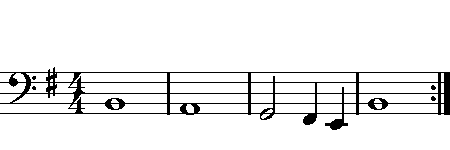
\includegraphics[width=2.7in]{Floyd-Bass-score.pdf}
    \end{center}

    \begin{figure}
        \centering
        \includegraphics[width=.98\textwidth]{Floyd-Guitar-Spectrum-0.png}
        \includegraphics[width=.98\textwidth]{Floyd-Guitar-Spectrum-1.png}
        \includegraphics[width=.98\textwidth]{Floyd-Guitar-Spectrum-2.png}
        \caption{The spectrogram of the second guitar solo in \textit{Comfortably Numb} by Pink Floyd. This range highlights the bass riff.}
        \label{fig:Floyd-Bass}
    \end{figure}

    The guitar riff comes out less desirably. The spectrogram is presented in figure \ref{fig:Floyd-Guitar}. I'm not able to write out a score as clearly as I did for the last two, but I can highlight a series of notes that should appear in the score in a certain order, basically a the score but missing some notes. This sequence is: $F4\sharp$, $E4$, $D5$, $B3$, $D5$, $F5\sharp$, $D5$, $B4$, $D5$, $E4$, $G4$, $D5$, $F5\sharp$, $A4$, $B3$, $F4\sharp$, $B4$, $E4$, $D5$.

    \begin{figure}[p]
        \centering
        \includegraphics[width=.98\textwidth]{Floyd-Bass-Spectrum-0.png}
        \includegraphics[width=.98\textwidth]{Floyd-Bass-Spectrum-1.png}
        \includegraphics[width=.98\textwidth]{Floyd-Bass-Spectrum-2.png}
        \caption{The spectrogram of the second guitar solo in \textit{Comfortably Numb} by Pink Floyd. This range highlights the guitar riff.}
        \label{fig:Floyd-Guitar}
    \end{figure}
    
    \section{Summary and Conclusions}
    % Summarize Gabor and How successful it was
    Using the Gabor transform, the spectrograms of the two clips were produced. For the guitar in \textit{Sweet Child O' Mine} and the bass in \textit{Comfortably Numb}, the notes are clearly identifiable. I have nearly an exact match between my score and the notes of published tabs \cite{GNR} \cite{Floyd}. The guitar solo in the Pink Floyd song was not clear enough to identify the score. That part of the spectrum suffered from severe pollution by the bass overtones. In addition, the solo as given by published tabs is much more complicated than the other two. What could be identified was an accurate subset of the song.

    % How successful was the bas filtering
    The bass was isolated with a low pass filter, which was very successful. The output file is almost entirely the sound of the bass. This was useful to confirming that the bass score was correct.

    \bibliographystyle{ieeetr}
    \bibliography{bibliography}
    \FloatBarrier
    \newpage
    \appendix
    This code is hosted on github \href{https://github.com/bagriffith/AMATH582/tree/main/HW2}{here}.
    \section{Python Functions}
    % Use PyDoc to generate
    \subsection{dmd}

\subsubsection{dmd}

\begin{Shaded}
\begin{Highlighting}[]
\NormalTok{dmd(X2, u, s, vh)}
\end{Highlighting}
\end{Shaded}

Returns the DMD modes and complex frequencies for the system.

\textbf{Arguments}:

\begin{itemize}
\tightlist
\item
  \texttt{X2} \emph{array-like} - The X\_2\^{}M matrix
\item
  \texttt{u} \emph{array-like} - The U matrix of the X\_1\^{}M-1 SVD
\item
  \texttt{s} \emph{array-like} - The s array of the X\_1\^{}M-1 SVD
\item
  \texttt{vh} \emph{array-like} - The vh matrix of the X\_1\^{}M-1 SVD
\end{itemize}

\textbf{Returns}:

\begin{itemize}
\tightlist
\item
  \texttt{ndarray} - Array of complex frequencies for DMD modes
\item
  \texttt{ndarray} - Matrix with rows of the DMD modes
\end{itemize}

\subsubsection{x\_dmd}

\begin{Shaded}
\begin{Highlighting}[]
\NormalTok{x_dmd(t, psi, w, b)}
\end{Highlighting}
\end{Shaded}

The DMD approximation of x(t).

\textbf{Arguments}:

\begin{itemize}
\tightlist
\item
  \texttt{t} \emph{float} - The time in frames
\item
  \texttt{psi} \emph{array-like} - Matrix with rows of the DMD modes
\item
  \texttt{w} \emph{array-like} - Array of complex frequencies for DMD
  modes
\item
  \texttt{b} \emph{array-like} - Array of initial values of the DMD
  modes
\end{itemize}

\textbf{Returns}:

\begin{itemize}
\tightlist
\item
  \texttt{ndarray} - DMD approximation of pixels at t
\end{itemize}

\subsubsection{frame\_bg\_sep}

\begin{Shaded}
\begin{Highlighting}[]
\NormalTok{frame_bg_sep(t, X, psi, w, b)}
\end{Highlighting}
\end{Shaded}

Separate the forground and background of frame t

\textbf{Arguments}:

\begin{itemize}
\tightlist
\item
  \texttt{t} \emph{int} - The time in frames
\item
  \texttt{psi} \emph{array-like} - Matrix with rows of the DMD modes
\item
  \texttt{w} \emph{array-like} - Array of complex frequencies for DMD
  modes
\item
  \texttt{b} \emph{array-like} - Array of initial values of the DMD
  modes
\end{itemize}

\textbf{Returns}:

\begin{itemize}
\tightlist
\item
  \texttt{ndarray} - Foreground array
\item
  \texttt{ndarray} - Background array
\end{itemize}

\subsubsection{show\_frame}

\begin{Shaded}
\begin{Highlighting}[]
\NormalTok{show_frame(frame, shape, path_out)}
\end{Highlighting}
\end{Shaded}

Plot the frame provided.

\textbf{Arguments}:

\begin{itemize}
\tightlist
\item
  \texttt{frame} \emph{array-like} - 1 D array of pixels
\item
  \texttt{shape} \emph{tuple} - The shape of the image (pixels\_y,
  pixels\_x)
\item
  \texttt{path\_out} \emph{str} - Path to save figure to
\end{itemize}

\subsection{svd}

\subsubsection{plot\_n\_modes}

\begin{Shaded}
\begin{Highlighting}[]
\NormalTok{plot_n_modes(X, V, n, shape, path_out)}
\end{Highlighting}
\end{Shaded}

Shows the numbers represented with the selected number of SVD modes

\textbf{Arguments}:

\begin{itemize}
\tightlist
\item
  \texttt{X} \emph{array\_like} - Data matrix with rows of images
\item
  \texttt{V} \emph{array\_like} - Matrix with mode vectors as columns
\item
  \texttt{n} \emph{int} - Number of modes to use in the representation
\item
  \texttt{shape} \emph{tuple} - The shape of the image (pixels\_y,
  pixels\_x)
\item
  \texttt{path\_out} \emph{str} - Path to save figure to
\end{itemize}

\subsubsection{plot\_mode\_fraction}

\begin{Shaded}
\begin{Highlighting}[]
\NormalTok{plot_mode_fraction(s, path_out)}
\end{Highlighting}
\end{Shaded}

Plots the fraction of power represented with n modes

\textbf{Arguments}:

\begin{itemize}
\tightlist
\item
  \texttt{s} \emph{array-like} - 1D arrray of the variances of the
  principal components.
\item
  \texttt{path\_out} \emph{str} - Path to save figure to
\end{itemize}

\subsection{loadVid}

\subsubsection{open\_video}

\begin{Shaded}
\begin{Highlighting}[]
\NormalTok{open_video(vid_path)}
\end{Highlighting}
\end{Shaded}

Loads the video matrices

\textbf{Arguments}:

\begin{itemize}
\tightlist
\item
  \texttt{vid\_path} \emph{str} - Path to the video file
\end{itemize}

\textbf{Returns}:

\begin{itemize}
\tightlist
\item
  \texttt{ndarray} - X\_1\^{}M-1
\item
  \texttt{ndarray} - X\_2\^{}M
\end{itemize}

    \section{Python Code}
    \subsection{spectrum.py}
    \inputminted{python}{../code/spectrum.py}


\end{document}
